\chapter{\system Implementation}
\label{chap:lazarus_implementation}

This chapter presents the \system solution and evaluation.
It implements the design described in the previous chapter in a centralized controller.
In addition, we also discuss an alternative implementation based on a distributed intrusion-tolerant controller.
\system currently manages 17 \gls{os} versions, supporting the \gls{bft} replication of a set of representative applications.
The replicas run in \glspl{vm}, allowing provisioning mechanisms to configure them in a fully automated way.
We conducted experiments that reveal the potential negative impact that virtualization and diversity can have on performance. 
However, we also show that if naive configurations are avoided, \gls{bft} applications in diverse configurations can perform close to our homogeneous bare metal setup.


\section{Implementation}
\label{sec:implementation}
\system is a control plane solution that collects data from \gls{osint} and uses this data to build diverse replica sets for \gls{bft} systems.
Over time, it monitors the \gls{osint} sources and the \gls{bft} replicas to enhance the failure independence of the replicas based on a risk metric.
Once the risk increases above a certain level, \system must replace replicas with different ones.
In this section, we detail the implementation of each component of \system. 
We also present other aspects and design decisions that were taken into account while building the prototype.% like the management of replicas running in a virtualized environment.


\subsection{Control Plane}
\label{sec:lazarus}

Figure~\ref{fig:arch1} shows \system control plane with its four main modules described below:

\begin{figure}[t]
\begin{center}
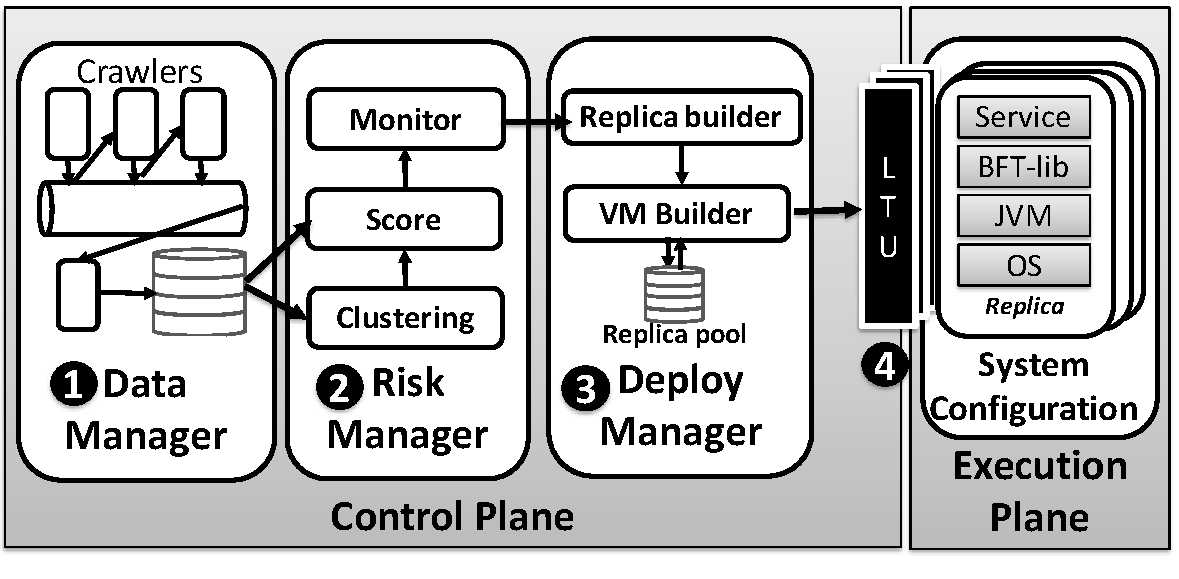
\includegraphics[width=.8\columnwidth]{images/images/architecture_new.pdf}
\caption{\system architecture.}
\label{fig:arch1}
\end{center}
\end{figure}



\circled{1} \textbf{\fetcher.} 
This component collects vulnerability data from several \gls{osint} sources and stores this data in a database to be analyzed by another \system component.
In particular, it only collects data for the software of interest.
We utilized the names included in the list of software products provided by the \gls{cpe} Dictionary~\cite{cpe}, which is also used by \gls{nvd}. 
Then, an administrator selects all the software that runs in each replica from this list and indicates the time interval (in years) during which data should be obtained from \gls{nvd}.
%\system needs to know the software stack of each available replica to be able to look for vulnerabilities in this software.
%The list of software products is provided by the CPE Dictionary~\cite{cpe}, which is also used by NVD. 
%The \fetcher determines if the CPE list is updated by checking the most recent CPE count in the NVD web page.
%For each software, the administrator can indicate the time interval (in years) during which data should be obtained from NVD feeds.
The \fetcher parses the \gls{nvd} feeds considering only the vulnerabilities that affect the chosen products. 
The processing is carried out with several threads cooperatively assembling as much data as possible about each vulnerability -- a queue is populated with requests pertaining a particular vulnerability, and other threads will look for related data in additional \gls{osint} sources. 
Typically, the other sources are not as well structured as \gls{nvd}, and therefore we had to develop specialized HTML parsers for them. 
Currently, the prototype supports eight other sources, namely Exploit DB~\cite{edb}, CVE-details~\cite{cvedetails}, Ubuntu~\cite{ubuntu}, Debian~\cite{debian}, Redhat~\cite{redhat}, Solaris~\cite{solaris}, FreeBSD~\cite{freebsd}, and Microsoft~\cite{microsoft}. 
%As previously mentioned, such sources provide complementary data, like additional affected products versions not mentioned in NVD.
The collected data is stored in a relational database (MySQL).
For each vulnerability, the manager keeps its \gls{cve} identifier, the published date, the products it affects, its text description, the \gls{cvss} attributes, exploit and patching dates.


\circled{2} \textbf{\risk.} This component finds out when it is necessary to replace the currently running group of replicas and discovers an alternative configuration that decreases the risk. 
As explained in Section~\ref{sec:measurerisk}, the risk is computed using score values that require two kinds of data: the information about the vulnerabilities, which is collected by the \fetcher, and the vulnerability clusters. 
A vulnerability cluster is a set of vulnerabilities that are related accordingly to their description.
We used the open-source machine learning library Weka~\cite{weka} to build these clusters. 
In a first phase, the vulnerability description needs to be transformed into a vector, where a numerical value is associated with the most relevant words (up to 200 words). 
This operation entails, for example, converting all words to a canonical form and calculating their frequency (less frequent words are given higher weights).
Then, the K-means~\cite{Jain:2010} algorithm is applied to build the clusters, where the number of clusters to be formed is determined by the elbow method~\cite{Thorndike:1953}.
%In our implementation the $K$ was set to $220$ clusters.
%The algorithm assigns each vulnerability to the cluster with the minimum distance to the cluster center. 
%Then, it computes the cluster centroid, i.e., the average of each data attribute using only the members of a cluster. 
%Next, it calculates the distance of every vulnerability to the centroid, potentially placing them in close clusters. 
%The algorithm stops when there are no further exchanges between clusters.
%We used the elbow method~\cite{Thorndike53whobelongs} to determine the number of clusters to be formed, in our case was $200$ clusters.
%We used the open-source machine learning library Weka~\cite{weka} to build the clusters. 

%The \risk also runs Algorithm~\ref{alg:algorithm2} to monitor the replicated system and trigger reconfigurations.


\circled{3} \textbf{\manager.} 
This component automates the setup and execution of the diverse replicas. 
It creates and deploys the replicas in the execution environment implementing the decisions of the \risk, i.e., it dictates when and which replicas leave and join the system. 
This sort of behavior must be initiated in a synchronous manner from a trusted domain. %, reducing the downtime of the service during the reconfigurations. 
One way to achieve this is to employ virtualization, leveraging on the isolation between the untrusted and the trusted domains~\cite{Sousa:2010,Platania:2014,Distler:2011}.
%Recovery triggering can be initiated from the isolated domain in a synchronous manner, reducing the downtime of the service during the reconfigurations. 
Therefore, we developed a replica builder on top of the Vagrant~\cite{vagrant} provisioning tool, which allows fast deployment of ready-to-use \glspl{os} and applications on \glspl{vm} (e.g., VirtualBox, VMware, and Docker).
%It supports several virtualization providers, such as VMware and Docker. 
From the available alternatives, we chose VirtualBox~\cite{virtualbox} because it supports a larger set of different guests \glspl{os}.


%It is responsible for downloading, installing, and configuring the \replicas.
%%%%Moreover, it performs replica maintenance, where  \replicas in \QS are booted to carry out automatic software updates (i.e., patching). 

\circled{4} \textbf{LTUs.} Each node that hosts a replica has a Vagrant daemon running on its trusted domain.
This component is isolated from the internet and communicates only with the \system controller through \gls{tls} channels.

\subsection{Execution Plane}
\label{sec:executionplane}

Despite the amount of relevant research on \gls{bft} protocols, only a few open-source libraries exist.
In theory, \system can use any of these, as long as they support replica set reconfigurations.
%In this case, it subsumes to the addition of a new replica and the removal of the old one.
More specifically, to manage the \replicas, we need the ability to add first a new \replica to the set and then remove the old \replica to be quarantined. 
Therefore, we employ \textsc{BFT-SMaRt}~\cite{Bessani:2014}, a stable \gls{bft} library that provides reconfigurations on the \replicas set.
The protocol we used can be briefly described as follows:
\emph{(i)} Once a new replica joins the group, it queries the other replicas about their last finished consensus instance;
\emph{(ii)} If the replica finds that the others also did not execute any instance, then no state transfer is required. 
Otherwise, the replica requests the state corresponding to the consensus instance it was in step \emph{(i)}.
\emph{(iii)} The other replicas verify if they have the state requested (i.e., a checkpoint and a log up to the specified consensus instance). 
If they do, they reply with the respective checkpoint and log -- only one replica sends a full checkpoint and the other $2f$ replicas send a hash of the checkpoint. 
Otherwise, they reply to the new replica with a void state.
\emph{(iv)} If the replica receives $2f+1$ matching replies for the requested state, it installs the received checkpoint and applies the operations in the log. 
If the $2f+1$ replies include a void state, the replica requests the state up to the consensus instance preceding the one being executed (thus beginning a new iteration of the protocol). 
This is repeated until the other replicas have the requested state. 



\subsection{Alternative Control Plane Design}
\label{sec:implementationdecisions}
So far we have been describing the \system control plane as a logically centralized component, and in fact, our current prototype is implemented as a single server (e.g.,~\cite{Roeder:2010,Platania:2014}).
This design was selected for two reasons.
First, it allowed us to focus on the main contributions of this work: runtime diversity assessment and performance.
Second, it matches the classical scenario where a single organization deploys an \emph{intrusion-tolerant service}~\cite{Verissimo:2003}, such as the managed (permissioned) blockchain services offered by major cloud providers (e.g., \cite{amazonblockchain,ibmblockchain}). 
In both scenarios, replica resources are already managed by a single organization that can host a \system control plane.

However, such design makes the controller a single point of compromise and prevents decentralized deployments where replicas are managed by different organizations.
In this section, we introduce an alternative approach based on a distributed intrusion-tolerant solution.
This solution envisions a set of servers, named \emph{controller replicas}, that run \system in a coordinated manner. 
Therefore, these servers can manage the replicas in the \emph{Execution Plane} as before and cooperate to keep the \emph{Control Plane} operational despite failures.
This version introduces some significant modifications to the previous architecture as illustrated in Figure~\ref{fig:lazarus_distributed}.
Moreover, a few changes were made on the system model, which are explained below.



\begin{figure}[t]
\begin{center}
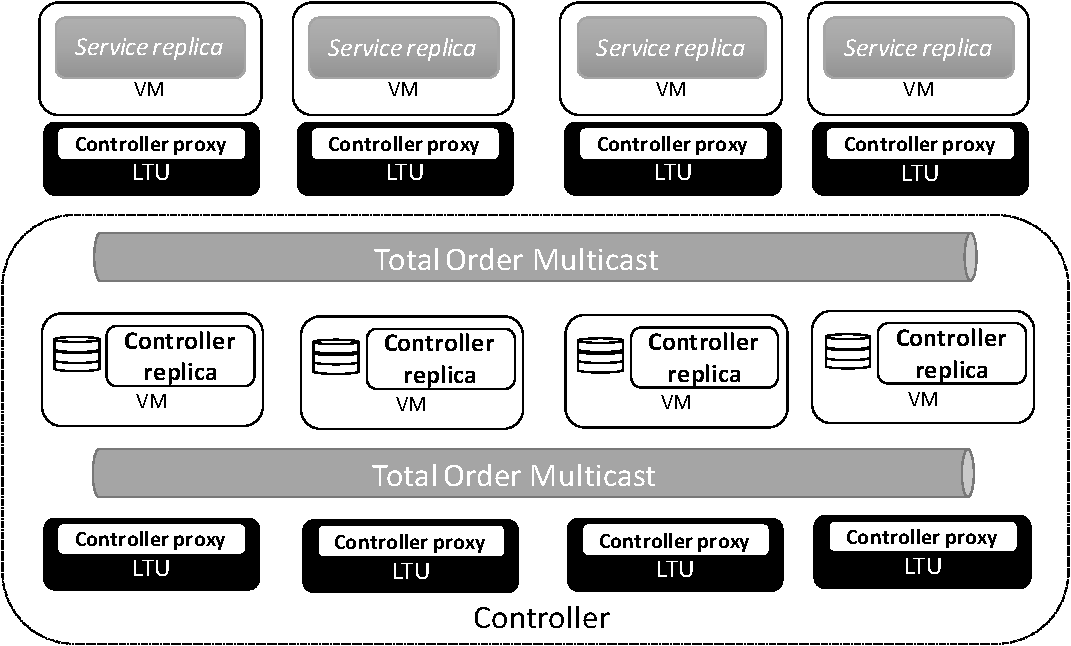
\includegraphics[width=0.9\columnwidth]{images/images/lazarus_distributed.pdf}
\caption{Distributed \system architecture.}
\label{fig:lazarus_distributed}
\end{center}
\end{figure}


\subsubsection{System Model}

This \system version attempts to minimize the changes to the centralized version.
For instance, the Execution Plane remains practically unmodified.
On the contrary, the Control Plane suffers some changes.
The new Control Plane is composed of replica processes, named \emph{controller replicas}, which can be subject to Byzantine failures.
Therefore, a Byzantine replica can try to mislead other replicas.
This plane hosts $n$ controller replicas from which at most $f$ can be compromised at any given moment.
Each replica has a \gls{ltu} co-located that is assumed to be trusted. 
The actions of this component cannot deviate from the expected behavior, which is especially important for the implementation of the recovery of replicas.


%\paragraph{Architecture.}

\subsubsection{Distributed Intrusion-tolerant Solution Challenges}
The design of a distributed intrusion-tolerant \system introduces a few modifications.
Most of these arise from the need to transfer the execution and storage logic from a single (and trusted) controller to $n$ replicated controllers.
In this process, we identify a few challenges:
(1) the need to ensure that a Service replica is asked to recover only when there is agreement among correct controller replicas;
(2) all controller replicas must have the same view of the database, thus, they need to collect \gls{osint} data in a synchronous way;
(3) in the \system monitoring algorithm a few decisions require a random selection, thus, in this version, all controller replicas must agree on the same random number without introducing biases;
(4) the replication of the controllers also brings storage problems, namely how to store the \gls{vm} images over the controllers;
and (5) applying patches on replicated \gls{vm} images introduces determinism problems as these images may not match after being patched.
In the following, we detail each challenge and provide possible solutions.
 
\paragraph{Recovery Protocol.}
Contrary to the centralized \system, where decisions to reconfigure are taken alone by the trusted controller, the replicated version needs a recovery protocol to ensure that a service replica is reconfigured if only and only if the operation was issued by correct controller replicas.
The communication between a \glspl{ltu} and the controller replicas is made via a total-order-multicast channel and it is used solely to trigger recoveries both on controller replicas and service replicas.
Each \gls{ltu} runs a controller proxy that can invoke controller replicas commands in a coordinated way, and it receives messages from controller replicas.
It has to wait for $f+1$ matching messages to know that the message is correct. 
Therefore, the controller proxy is ready to trigger a recovery on a service replica or on a controller replica.
Contrary to the usual request-response of \gls{smr}, here, the controller proxy receives ``responses'' without a prior request. 


\paragraph{Replica Synchronization Protocol.}
In its centralized version, a single \system controller takes decisions alone.
For example, it decides when it is the time to contact \gls{osint} sources to look for new data, or when it is the time to substitute service replicas.
On the contrary, in a distributed setup, the replicas must be coordinated to execute the same command \emph{at the same time}.
One way to do that is to assume that replicas have synchronous clocks, and then, all the requests are synchronized.
However, we want to make as few time assumptions as possible.
Moreover, by using the internet to communicate with \gls{osint} sources, \system communication is subject to different levels of delays.
Therefore, we propose a solution that uses a logical timeout protocol to (logically) synchronize replicas.
This protocol was proposed by Kirsch~\etal{}~\cite{Kirsch:2014} to coordinate replicas on polling requests to a sensor in the context of \gls{scada} systems.
The decentralized \system can employ this protocol to guarantee that all controller replicas poll \gls{osint} at the same logical time.
This protocol can be described in the following way:
All controller replicas run an algorithm that periodically sends a \texttt{SYNC} message among them.
This message is used to inform other replicas of the current timeouts that a controller replica has.
Each controller replica will set their own timeouts by setting up a timeout \texttt{T$_x$} with the local time \emph{c$_i$} and the local expiration time \emph{$d$} to a controller replica \emph{i}, where $i \in \{1, ..., n\}$.
Then, it sends to the others the \emph{$c_i$} and \emph{$d$} within a \texttt{SYNC} message.
This allows every replica to update their own list of timeouts, and each one sets the expiration time as \emph{$c_i + d$} for \texttt{T$_x$}.
When a \texttt{SYNC} message from $i$ says that the local clock is greater than \emph{$c_i + d$}, then the timeout \texttt{T$_x$} was expired.
When a logical timeout is triggered in $f+1$ different controller replicas, the timeout \texttt{T$_x$} is delivered to the application.
In this way, it is guaranteed that replicas will poll \gls{osint} sources only when $f+1$ controller replicas had \texttt{T$_x$} expired.
 


\paragraph{Distributed Random Generation Protocol.}
As explained in Chapter~\ref{chap:lazarus_design}, \system selects random configurations to prevent attackers from guessing which will be the next configuration.
In the centralized version of the system, it is simple to select random values.
However, random number generation is a challenge for distributed systems.
In particular, it is difficult to determine a random value among the replicas without prior knowledge of anyone and guaranteeing that the random value is not biased, i.e., that a malicious replica is not influencing the final value.
There are already algorithms that can be employed to address this problem.
For example, RandShare~\cite{Syta:2017} ensures unbiasability, unpredictability, and availability on random number generation.
The protocol was developed in such a way that after a protocol barrier, honest replicas will eventually output the previously decided value despite the adversary's behavior.
The protocol uses secret sharing~\cite{Shamir:1979} and polynomial commitments to create shares of a local random number and distributes them among the peers.
With the polynomial commitment, a replica is able to verify if the share is valid without revealing information about the secret.
When all their verifications are made, each replica informs the others about the validations, then any peer knows all the validations done by the others.
After this stage, all replicas can recover the secrets via Lagrange interpolation.
Finally, the random number is generated through a \texttt{xor} operation with the different recovered secrets.


\paragraph{Distributed Storage.}
Another modification that we have identified is the storage location. 
In a centralized solution, the storage is a single pool that is accessed by the controller.
A straw-man solution would be to use full replication of the pool and each controller proxy would wait for $f+1$ responses (the actual replica image and a cryptographic hash of the image to verify).
However, this solution is not resource efficient as it requires that all replica images be copied on all controller replicas.
A more sophisticated solution would take advantage of erasure codes (e.g.,~\cite{Reed:1960}) with secret sharing.
This approach would minimize the use of resources, as each controller replica would store only parts of the complete image.
Moreover, it would simplify the recovery of these replicas as they would only need to recover parts of the original image instead of the complete image.
Nevertheless, this approach implies additional complexity on the controller proxy as it needs to rebuild the blocks and verify them.


\paragraph{Deterministic Image Patching.}
One of the main problems that the distributed solution brings is to guarantee that the images are loaded in a deterministic way.
\gls{smr} requires that the replicas start from an equal state and apply the same operations to the state in such a way that the replicas reply with the equivalent answers to the clients.
Therefore, it is a challenge to create \gls{vm} images that have exactly equal binaries. 
Moreover, once a replica is patched it becomes hard to ensure that it is equal across the controller replicas and this can prevent appropriate voting operations. 
%Therefore, once a Controller proxy that is responsible to load a \gls{vm} (in the Execution Plane) cannot vote which image is correct as they are different among the (even correct) Controller replicas due to the patches. 
For the moment, the proposed solution is to rely on a trusted \gls{vm} maintainer whose role is to update and distribute the \gls{vm} images through the different controller replicas. 
In this way, every controller replica receives the same \gls{vm} image.


\section{Application and Parameter Details}

In this section, we detail some configuration and parameters used on the \system components. 
First, we describe each step of the clustering process.
Then, we explain how the replicas are built using the Vagrant provisioning tool.


\subsection{Clustering}\label{sec:clustering}

Clustering is the process of aggregating the different elements into groups, which are named clusters. 
The aim is to ensure that two elements from the same cluster have a higher probability of being similar than two elements from different clusters. 
We apply this technique to build clusters of vulnerability entries in our database.
One of the benefits of applying clustering techniques to information about vulnerabilities is that the algorithm does not need prior knowledge about the data.
It is the process alone that discovers the hidden knowledge in the data.
Each cluster is used as a hint that similar vulnerabilities are likely to be activated through the same (or near identical) exploit.
We considered the vulnerability description and published date to build the clusters. 
In the end, it is expected that clusters have a minimal number of elements that represent approximately the same vulnerability.


A few steps are carried out to create the vulnerability clusters. 
First, the vulnerability description needs to be transformed into a vector, where a numerical value is associated with the most relevant words. 
This operation entails, among other tasks, converting all words to a canonical form and calculating their frequency (less frequent words are given higher weights).
Then, the clustering algorithm is applied to aggregate the vulnerabilities. 
We used the open-source machine learning library Weka~\cite{weka} to prepare the data and build the clusters as described in the following:



\paragraph{1) Data representation}
We transform the data that is stored in the database into a format that is readable by the clustering algorithm. 
Since we are using Weka, the data must be represented in the \gls{arff}. 
Basically, this is a CSV file with some meta data information as exemplified in Listing~\ref{list:arff}.


This file contains all the vulnerabilities entries in the database. 
As we are interested in the vulnerability similarities, we select only the \gls{cve} identifier, the text (as it contains the most relevant and nonstructured information) and the published date.
These attributes add meaning and temporal reference to the clustering algorithm.

\begin{lstlisting}[style=mystyle,caption=ARFF file describing a vulnerability.,label=list:arff]
@RELATION vulnerabilities
@ATTRIBUTE cve string
@ATTRIBUTE description string
@ATTRIBUTE published_date date "yyyy-MM-dd"
@DATA
CVE-2017-3301, 'vulnerability in the solaris component of oracle sun systems products suite subcomponent kernel the supported version that is [...] attacks of this vulnerability can result in unauthorized update insert or delete access to some of solaris accessible data cvss base score integrity impacts', '2017-01-27'
...more
\end{lstlisting}


\paragraph{2) Data preparation}
In general, machine learning algorithms do not handle raw information, and therefore the data needs to be prepared:
First, we transform the \gls{cve} string into a number, ensuring that there is a real number that corresponds to each \gls{cve} unequivocally. 
This attribute is translated into a numeric value using the \emph{StringToNominal} filter. 
Second, we also transform the published date into a number format using the \emph{NumericToNominal} filter.
Third, the text description must be transformed into a vector representation using the \emph{StringToWordVector} filter.
This vector has the frequencies of each word in the whole text description. 
A few steps are taken in this filtering process. 
First, all the words are converted to lower case and certain special characters are removed to reduce the noise and differences among the words. 
From this sequence of words only the ones that are not in the stop word list (e.g., a, an, the) are kept.
Then, it the TF- and IDF-Transform~\cite{Leskovec:2014} is used to measure how relevant a word is to a vulnerability entry in the whole collection. 
The relevance increases proportionally to the number of times a word appears in the vulnerability description but is offset by the frequency of the word in the whole body of text. 
For example, words that appear in all vulnerability descriptions, are less relevant than the ones that appear only in few vulnerabilities.
In the end, only a pre-defined number of words is saved. 
In our current implementation, we empirically found that $200$ is the best number of words to represent the description of vulnerabilities after removing the \emph{stopwords}.

%This filter contains the following parameters:
%\begin{itemize}
%\item \textbf{TF- and IDF-Transform}, both set to true, TF-IDF stands for term frequency-inverse document frequency. 
%This is a statistical measure used to evaluate how relevant a word is to a document in a collection. 
%The relevance increases proportionally to the number of times a word appears in the document but is offset by the frequency of the word in the corpus. 
%For example, words that appear in all vulnerability descriptions, are less relevant than the ones that appear more in few vulnerabilities.
%\item \textbf{lowerCaseTokens}, convert all the words to lower case.
%\item \textbf{minTermFreq}, set to -1, this will preserve any word despite their occurrences in the document.
%\item \textbf{normalizeDocLength}, set to normalize all data counting a word with its actual value from TF-IDF no matter how small or longer the document is.
%\item \textbf{stopwords}, we define a stop word list, then words from this list are discarded. We begin with a generic English stop word list containing pronouns, articles, etc. 
%\item \textbf{tokenizer}, set to \emph{WordTokenizer}, this filter will remove special characters from the text, there is a default set of characters, but we added a few more.
%\item \textbf{wordsTopKeep}, is the number of words that will be kept to make the clusters. We kept $200$ as it was the number of words that represent better the lexical of %vulnerabilities after removing the \emph{stopwords}.%
%\end{itemize}


Our goal is to build clusters in such a way that similar vulnerabilities, even if they affect different products, are put together in the same group. 
For instance, recall the example vulnerabilities in Table~\ref{tab:missing_products}, which should be placed together in the same cluster as they are alike.
To achieve this, some of the parameters listed above had to be tuned.
We observed that before the tuning, some of the clusters were very generic representing large classes of vulnerabilities, e.g., buffer overflow and cross-site scripting. 
Since we are not interested in this sort of classification, we have refined the \emph{stopword list} to make the description vocabulary contain only what matters for our goal.
This was done by checking an intermediary Weka's output that shows the most used words to build the clusters.
Then, we picked the most relevant words from this list and added them to the stop word list to prevent the creation of clusters by vulnerability class.


When the pre-filtering ends, Weka presents a file, similar to the previous \gls{arff} file, where the features represent the relevance of the words of all description texts for each entry as shown in Listing~\ref{list:arff2} (e.g., apache is more relevant in CVE-2017-5884 description than in CVE-2015-0001). 

\begin{lstlisting}[style=mystyle,caption=ARFF file after data preparation.,label=list:arff2]
@relation 'vulnerabilities-weka.filters.unsupervised.attribute.Remove-R3-weka.filters.unsupervised.attribute.StringToNominal ..more

@attribute cve {CVE-2017-3301,CVE-2017-5884,CVE-2015-0001 ...more}
@attribute access numeric
@attribute application numeric
@attribute apache numeric
@attribute arbitrary numeric
...more 
@data
{CVE-2017-5884, 0.212441,6 0.1924,10 1.3516,15 0.527593,21 1.550981  ...more }
{CVE-2015-0001, 0.930885,6 0.12374,8 0.347466,10 0.869272,17 1.088708 ...more }
...more
\end{lstlisting}




\paragraph{3) Building the clusters}
K-means is an unsupervised machine learning algorithm that groups data in K clusters~\cite{Jain:2010}.
This algorithm has two important parameters: the number of clusters to be formed and the \emph{distance function} used to calculate the distance between each data entry.
The K-means computes the distance from each data entry to the cluster center (randomly selected in the first round).
Then, it assigns each data entry to a cluster based on the minimum distance (i.e., Euclidean distance) to each cluster center.
Then, it computes the centroid, that is the average of each data attribute using only the members of each cluster.
Next, it calculates the distance from each data entry to the recent centroids. 
If there is no modification (i.e., re-arrangement of the entries in the cluster), then the clusters are complete. 
Otherwise, it recalculates the distance that best fits the elements. 
When the K-means finishes the execution, we take the cluster assignments of each vulnerability. 
The assignments will be added to a new \gls{arff} file, similar to the first one but with a new attribute that is the cluster name (e.g., cluster1, cluster2). 
In our setup, we used the elbow method~\cite{Thorndike:1953} to decide K$=220$.


%Sometimes the resulting clusters include vulnerabilities that are unrelated. Therefore, we use the Jaccard index (J-index) to measure the similarity between the vulnerabilities within the cluster. We calculate the J-index of each element, and then the average J-index of the cluster. 
%The clusters with a smaller average J-index (below a certain threshold) are considered ill-formed. In this case, we select the vulnerabilities with lower J-index and move them to another cluster that would result in a better J-index. If no such cluster exists, then we create a new one with the ``orphan'' vulnerability.


\subsection{Replica Virtualization and Provision}
In this section we describe the parameters and configurations used to implement the \manager with the support of Vagrant and Virtualbox.

\paragraph{Setup.}
A \gls{vm} configuration is defined in a file, named \emph{Vagrantfile}, as displayed in the example of Listing~\ref{vagrantfile}.
In this file, it is possible to set all the options to build a \gls{vm}, like:
the number of CPUs, the amount of memory RAM, the IP, the type of network, and the sync folders between the host and the \gls{vm}.
Since Vagrant supports different \gls{vm} providers (e.g., libvirt, VMware, VirtualBox, Parallels, Docker, etc), we selected VirtualBox as displayed in line 4 of Listing~\ref{vagrantfile}.
Additionally, it is also possible to pass some VM-specific parameters, namely the CPU/mother board flags that enable for instance the VT-x technology -- consider the \texttt{modifyvm} fields in Listing~\ref{vagrantfile} (lines 8-13).

% we rely on VirtualBox since it is the one with more diversity opportunities in the Vagrant Cloud~\cite{vagrantcloud}. 
%Vagrant Cloud is a website that offers a plethora of different \glspl{vm}.

\begin{lstlisting}[style=mystyle,caption=Ubuntu 16.04 Vagrantfile,label=vagrantfile]
Vagrant.configure(2) do |config|
	config.vm.box = "geerlingguy/ubuntu1604"
	config.ssh.insert_key = false
	config.vm.provider "virtualbox" do |v|
		v.customize ["modifyvm", :id, "--cpus", 4]
		v.customize ["modifyvm", :id, "--memory", 22000]
		v.customize ["modifyvm", :id, "--cpuexecutioncap", 100]
		v.customize ["modifyvm", :id, "--ioapic", "on"]
		v.customize ["modifyvm", :id, "--hwvirtex", "on"]
		v.customize ["modifyvm", :id, "--nestedpaging", "on"]
		v.customize ["modifyvm", :id, "--pae", "on"]
		v.customize ["modifyvm", :id, "--natdnshostresolver1", "on"]
		v.customize ["modifyvm", :id, "--natdnsproxy1", "on"]
	end
	config.vm.network "public_network", ip:"192.168.2.50", bridge:"em1"
	config.vm.provision :shell, path: "run_debian.sh", privileged: true
end
\end{lstlisting}


\paragraph{Download.}
One of the fields of the Vagrantfile is the \texttt{box} field, which identifies the \gls{os} release that will be downloaded -- line 2 in Listing~\ref{vagrantfile}.
There are many of \glspl{os} and versions ready-to-use, and the same \gls{os}/version can have different manufacturers -- some of which are made available by the vendor itself.

\paragraph{Deploy and provision.}
Although Vagrant supports complex provisions mechanisms, such as Chef or Puppet, a shell script was sufficient for us. 
This parameter is set in the Vagrantfile \texttt{provision} field, where one puts the path to the script file -- line 16 in Listing~\ref{vagrantfile}.
Then, when the \gls{os} is booting, the \glspl{os} will execute the provision script after the basic setup.
In this script, we define which software will be downloaded and run in the \glspl{vm} and what configurations are needed. 
We have developed shell scripts for each \gls{os}, some of which shared as in Debian and Ubuntu. 
Since \glspl{os} have different commands to execute the same instructions, it is necessary to customize these scripts.
These scripts install software like Java 8, \texttt{wget}, \texttt{unzip}, and any additional packages that one wants to install/run after the \gls{os} boot.



\paragraph{Command and Control.}
There are some simple commands to boot and halt a \gls{vm}, e.g., \texttt{vagrant up} and \texttt{vagrant halt}. 
Vagrant also provides a secure shell command (\texttt{vagrant ssh}) that allows the host to connect to the \gls{vm}. 
Our manager component makes the bridge between the \risk and the execution environment.
We developed an API on top of Vagrant to allow replica management.



\section{Evaluation}
\label{sec:overhead}

In this section, we evaluate the performance of \system while managing diverse replicated systems.
First, we run the \textsc{BFT-SMaRt} microbenchmarks in our virtualized environment to understand how the performance of a \gls{bft} protocol varies with different \glspl{os}.
In addition, we compare the performance of the virtualized deployment with an homogeneous bare metal setup.
Second, we use the same benchmarks to measure the performance of specific diverse setups (e.g., the fastest and slowest set of \glspl{os}).
Third, we analyze the overheads introduced in the system by the \system-managed reconfigurations.
In particular, we measure the time it takes for each \gls{os} to boot.
Finally, we evaluate the performance of three \gls{bft} services running in the \system infrastructure.


These experiments were conducted in a cluster of Dell PowerEdge R410 machines, where each one has 32 GB of memory and two quad-core 2.27 GHz Intel Xeon E5520 processors with hyper-threading, i.e., supporting 16 hardware threads on each node.
The machines communicate through a gigabit Ethernet network.
Each server runs Ubuntu Linux 14.04 LTS (3.13.0-32-generic Kernel) and VirtualBox 5.1.28, for supporting the execution of \glspl{vm} with different \glspl{os}. 
Additionally, Vagrant 2.0.0 was used as the provisioning tool to automate the deployment process.
In all experiments, we configure \textsc{BFT-SMaRt} v1.1 with four replicas ($f=1$), one replica per physical machine.

\begin{table}[t]
\begin{center}
{\footnotesize
\begin{tabular}{| c | c | c | c | c |}\hline
\textbf{ID} & \textbf{Name}  & \textbf{Cores} & \textbf{JVM} & \textbf{Mem.} \\\hline\hline
UB14 & Ubuntu 14.04 & 4 & Java Oracle 1.8.0\_144 & 15GB \\ \hline
UB16 & Ubuntu 16.04 & 4 & Java Oracle 1.8.0\_144 & 15GB \\ \hline
UB17 & Ubuntu 17.04 & 4 & Java Oracle 1.8.0\_144 & 15GB \\ \hline
OS42 & OpenSuse 42.1 & 4 & Openjdk 1.8.0\_141 & 15GB \\ \hline
FE24 & Fedora 24 & 4 & Openjdk 1.8.0\_141 & 15GB \\ \hline
FE25 & Fedora 25 & 4 & Openjdk 1.8.0\_141 & 15GB \\ \hline
FE26 & Fedora 26 & 4 & Openjdk 1.8.0\_141 & 15GB \\ \hline
DE7 & Debian 7 & 4 & Java Oracle 1.8.0\_151 & 15GB \\ \hline
DE8 & Debian 8 & 4 & Openjdk 1.8.0\_131 & 15GB \\ \hline
W10 & Windows 10 & 4 & Java Oracle 1.8.0\_151 &1GB \\ \hline
WS12 & Win. Server 2012 & 4 & Java Oracle 1.8.0\_151 & 1GB \\ \hline
FB10 & FreeBSD 10 & 4 & Openjdk 1.8.0\_144 & 15GB \\ \hline
FB11 & FreeBSD 11 & 4 & Openjdk 1.8.0\_144 & 15GB \\ \hline
SO10 & Solaris 10 & 1 & Java Oracle 1.8.0\_141 & 15GB \\ \hline
SO11 & Solaris 11 & 1 & Java Oracle 1.8.0\_05 & 15GB \\ \hline
OB60 & OpenBSD 6.0 & 1 & Openjdk 1.8.0\_72 & 1GB \\ \hline
OB61 & OpenBSD 6.1 & 1 & Openjdk 1.8.0\_121 & 1GB \\ \hline
\end{tabular}
}
\vspace{2mm}
\caption{The different OSes used in the experiments and the configurations of their VMs and JVMs.}
\label{tab:oses}
\end{center}
\end{table}

Table~\ref{tab:oses} lists the 17 \gls{os} versions used in the experiments and the number of cores made available to their corresponding \glspl{vm}.
These values correspond to the maximum number of CPUs supported by VirtualBox with that particular \gls{os}.
The table also shows the \gls{jvm} used in each \gls{os}, and the amount of memory supported by each of these \glspl{vm}.
Given these configurations we setup our environment to establish a fair baseline by setting up an \emph{homogeneous} \gls{bm} environment that uses only four cores of the physical machine. 

%Given the limitations of the VMs we were able to setup in our environment, all experiments conducted in our \emph{homogeneous bare metal environment} (BM) were configured to make BFT-SMaRt replicas use only four cores of the machines, to establish a fair baseline.



\subsection{Homogeneous Replicas Throughput}

We start by running the \textsc{BFT-SMaRt} microbenchmark using the \emph{same \gls{os} version} in all replicas.
The microbenchmark considers an empty service that receives and replies variable size payloads, and is commonly used to evaluate \gls{bft} state-machine replication protocols (e.g., \cite{Castro:1999,Bessani:2014,Liu:2016,Behl:2015,Behl:2017}). 
Here, we consider the $0/0$ and $1024/1024$ workloads, i.e., $0$ and $1024$ bytes requests/response, respectively.
The experiments employ up to 1400 client processes spread on seven machines to create the workload.
% and the throughput was measured in the BFT-SMaRt leader replica.

\begin{figure}[t]
\begin{center}
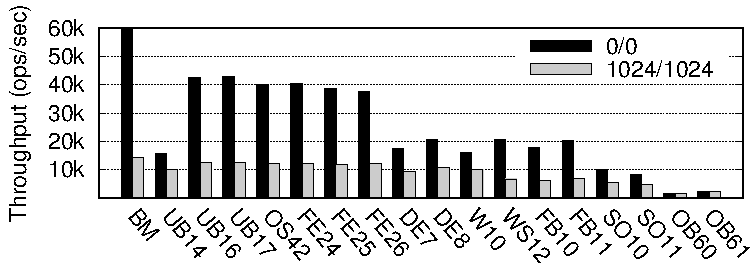
\includegraphics[width=\columnwidth]{images/gnuplot/vagrant/runs_new_new/throughput.pdf}
\caption{Microbenchmark for 0/0 and 1024/1024 (request/replying) for homogeneous OSes configurations.}
\label{fig:bftsmart}
\end{center}
\end{figure}


\textbf{Results:}
Figure~\ref{fig:bftsmart} shows the throughput of each \gls{os} running the benchmark for both loads.
To establish a baseline, we also executed the benchmark in our bare metal Ubuntu, without \system virtualization environment.

The results show that there are some significant differences between running the system on top of different \glspl{os}.
This difference is more significant for the $0/0$ workload as it is much more CPU intensive than the $1024/1024$ workload.
Ubuntu, OpenSuse, and Fedora OSes are well supported by our virtualization environment and achieved a throughput around $40k$ and $10k$ ops/sec for the $0/0$ and $1024/1024$ workloads, which corresponds to approx. $66\%$ and $75\%$ of the bare metal results, respectively.
For Debian, Windows, and FreeBSD, the results are much worse for the CPU-intensive $0/0$ workloads but close to the previous group for $1024/1024$.
Finally, single core \glspl{vm} running Solaris and OpenBSD reached no more than $3000$ ops/sec with both workloads.

These results show that the virtualization platform introduces a few limitations on supporting different \glspl{os}, and strongly constrains the performance of specific \glspl{os} in our testbed.


\subsection{Diverse Replicas Throughput}
\label{sec:performancediversity}

The previous results show the performance of \textsc{BFT-SMaRt} when running on top of different \glspl{os}, but with all replicas running in the same environment.
In this experiment, we evaluate three diverse sets of four replicas, one with the fastest \glspl{os} (UB17, UB16, FE24, and OS42), another with one replica of each \gls{os} family (UB16, W10, SO10, and OB61), and a last one with the slowest \glspl{os} (OB60, OB61, SO10, and SO11).
The idea is to set an upper and lower bound on the throughput of all possible diverse replica sets.

\begin{figure}[t]
\begin{center}
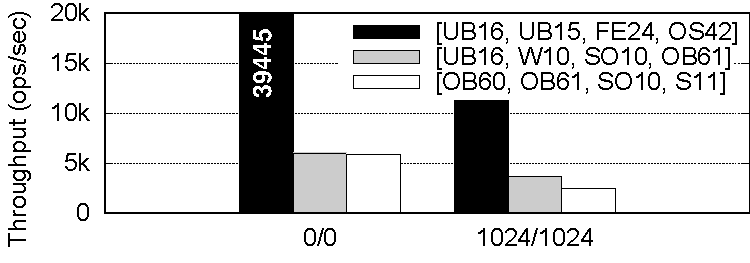
\includegraphics[width=0.8\columnwidth]{images/gnuplot/vagrant/runs_diversity/throughput.pdf}
\caption{Microbenchmark for 0/0 and 1024/1024 (request/reply) for three diverse OS configurations.}
\label{fig:diversets}
\end{center}
\end{figure}


\textbf{Results:}
Figure~\ref{fig:diversets} shows that throughput drops from $39k$ to $6k$ for the $0/0$ workload ($65\%$ and $10\%$ of the bare metal performance), and from $11.5k$ to $2.5k$ for the $1024/1024$ workload ($82\%$ and $18\%$ of the bare metal performance).
When comparing these two setups with the non-diverse configurations of Figure~\ref{fig:bftsmart}, the fastest set is in $7^{th}$, and the slowest set is in $16^{th}$ in terms of the achieved throughput.
It is worth to stress that the slowest set is composed of \glspl{os} that only support a single CPU -- due to the VirtualBox limitations -- therefore the low performance is somewhat expected.
The set with \glspl{os} from different families is very close to the slowest set, as two of the replicas use single-CPU \glspl{os}, and \textsc{BFT-SMaRt} always makes progress at the speed of the 3rd fastest replica (a Solaris \gls{vm}), since its Byzantine quorum needs three replicas for ordering the requests.
These results show that running \system with current virtualization technology results in a significant performance variation, depending on the configurations selected by the system.
This opens interesting avenues for future work on protocols that consider such performance diversity, as will be discussed in Chapter~\ref{chap:conclusion}.

\subsection{Performance During Replicas' Reconfiguration}
\label{sec:reconfiguration}
Another relevant feature of \system is to adapt the replicas over time. 
\system leverages on the \textsc{BFT-SMaRt} reconfiguration protocol~\cite{Bessani:2014} to add and remove replicas while \gls{bft} state is maintained correct and up to date.

In this experiment, we want to compare the replicas reconfiguration in the homogeneous \gls{bm} environment with the \system environment (the initial \gls{os} configuration is DE8, OS42, FE26, and SO11).
Our goal is to evaluate the two different environments with the same experimental setup to measure the overhead of \system-induced reconfigurations. 
We execute this experiment with an in-memory \gls{kvs} service that comes with the \textsc{BFT-SMaRt} library.
The experiment was conducted with a \gls{ycsb}~\cite{Cooper:2010} workload of $50\%$ of reads and $50\%$ of writes, with values of $1024$ bytes associated with small numeric keys, varying the state size of the \gls{kvs}.
Since the virtualization environment limits the performance (as shown in the previous experiments), we used a workload that best fits both environments.
Then we setup the benchmark to send $\approx 4000$ operations per second over a state of $500$MBs. 
We selected a time frame of $200$ seconds to show the performance during a reconfiguration.


\begin{figure}[t]
\begin{center}
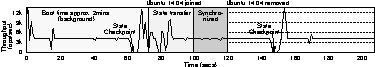
\includegraphics[width=\textwidth]{images/gnuplot/vagrant/reconfiguration/reconfiguration_bm.pdf}
\caption{Bare Metal reconfiguration KVS performance on a 50/50 YCSB workload, 1kB-values and with $\approx 500$MBs state size.}
\label{fig:reconfiguration_bm}
\end{center}
\end{figure}
\begin{figure}[t]
\begin{center}
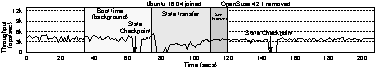
\includegraphics[width=\textwidth]{images/gnuplot/vagrant/reconfiguration/reconfiguration_vm.pdf}
\caption{\system reconfiguration KVS performance on a 50/50 YCSB workload, 1kB-values and with $\approx 500$MBs state size..}
\label{fig:reconfiguration_vm}
\end{center}
\end{figure}

\textbf{Results:}
Figures~\ref{fig:reconfiguration_bm} and ~\ref{fig:reconfiguration_vm} show the replicas throughput measured with \gls{ycsb} benchmark which runs in the client side. 
In both figures, there are two types of performance drops. 
The first one, named state checkpoint, is the period in which the \textsc{BFT-SMaRt} replicas trim their operation logs.
During these periods there are no messages processed. 
%Nevertheless, for states smaller than $50$MBs there is only a slight decrease in the throughput.
The second ones, composed of the state transfer and the synchronization, were already identified, and mitigated in previous works~\cite{Bessani:2013}.\footnote{We employ the standard checkpoint and state transfer protocols of \textsc{BFT-SMaRt} and not the ones introduced in~\cite{Bessani:2013} as it is more stable.}  

There are some differences between both executions, in particular, the throughput variation and the time each phase takes to finish.
Both experiments were made to represent the same behavior, therefore the different actions start approximately at the same time.
For example, in both cases, the state checkpoint is made almost at the same time as it is triggered by the number of processed messages on each replica.

In the BM experiment (Figure~\ref{fig:reconfiguration_bm}) the state checkpoint occurs around the second $60$.
After a few seconds, the new replica (i.e., Ubuntu 14.04) joins the system, and a state transfer begins.
It takes almost $30$ seconds to get the state and then it takes approx.~$20$ seconds to execute the log and reach the other replicas state. 
Only then one of the \emph{old} replicas is removed. 
The booting time for Ubuntu 14.04 was more than $2$ mins in our testbed.\footnote{This time is due to special verification tests that machines in a cluster typically do before booting.} 

\begin{figure}[t]
\begin{center}
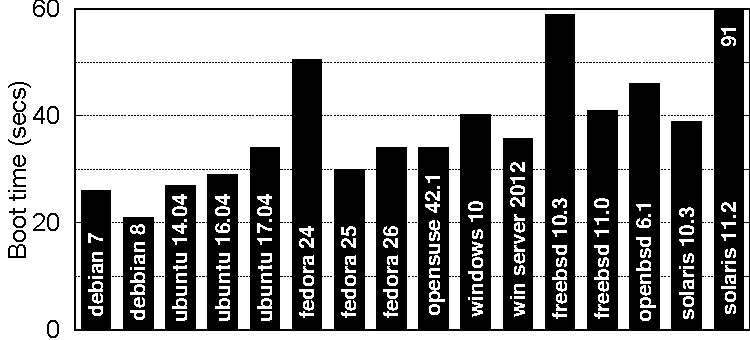
\includegraphics[width=0.8\columnwidth]{images/gnuplot/vagrant/updown/boot.pdf}
\caption{OSes boot times (seconds).}
\label{fig:boot}
\end{center}
\end{figure}

In the \system setting experiment (Figure~\ref{fig:reconfiguration_vm}), it is possible to see a little variance on the throughput overall but it has a significant impact during the reconfiguration. 
However, the throughput and the time it takes to finish the state reconfiguration is close to the previous experiment.
Finally, the booting takes approx.~$40$ seconds.

Additionally, we have conducted a more straightforward experiment to measure the boot time of the \glspl{os} supported by \system prototype. 
Figure~\ref{fig:boot} shows the average boot time of $20$ executions boot for each \gls{os}.
As can be seen, most \glspl{os} take less than $40$ seconds to boot, with the exceptions of Fedora 24 ($50$ seconds), FreeBSD 10.3 ($59$ seconds), and Solaris 11.2 ($91$ seconds).
In any case, these results together with the reconfiguration times of the previous section show that \system can react to a new threat in less than two minutes (in the worst case).
\subsection{Application Benchmarks}
Our last set of experiments aims to measure the throughput of three existing \gls{bft} services built on top of \textsc{BFT-SMaRt} when running in \system.
The considered applications and workloads are:

\begin{itemize}

\item \emph{KVS} is the same \textsc{BFT-SMaRt} application employed in Section~\ref{sec:reconfiguration}.
It represents a consistent non-relational database that stores data in memory, similarly to a coordination service (an evaluation scenario used in many recent papers on \gls{bft}~\cite{Liu:2016,Behl:2017}).
In this evaluation, we employ the \gls{ycsb} $50\%/50\%$ read/write workload with values of 4k bytes.

\item \sieveq~\cite{Garcia:2016} was presented in detail in Chapter~\ref{chap:sieveq}. In this evaluation, we consider that all the layers were running on the same four physical machines as the diverse \textsc{BFT-SMaRt} replicas (under different \glspl{os}).
The workload imposed on the system is composed of messages of 1k bytes.

\item \emph{BFT ordering for Hyperledger Fabric}~\cite{Sousa:2018} is the first \gls{bft} ordering service for Fabric~\cite{Androulaki:2018}. 
Fabric is an extensible blockchain platform designed for business applications beyond the basic digital coin.
The ordering service is the core of Fabric, being responsible for ordering and grouping issued transactions in signed blocks that form the blockchain.
In our evaluation, we consider transactions of 1k bytes, blocks of $10$ transactions and a single block receiver.

\end{itemize}

As in Section~\ref{sec:performancediversity}, we run the applications on the fastest and slowest diverse replica sets and compare them with the results obtained in bare metal.

\begin{figure}[t]
\begin{center}
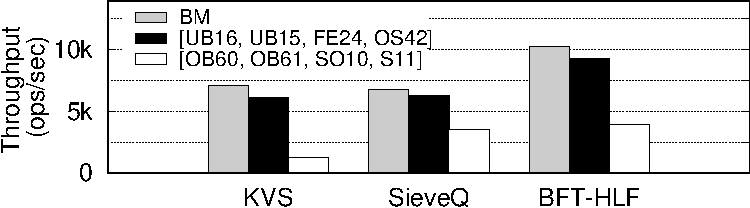
\includegraphics[width=0.8\columnwidth]{images/gnuplot/vagrant/runs_apps/throughput.pdf}
\caption{Different BFT applications running in the bare metal, fastest and slowest OS configurations.}
\label{fig:apps}
\end{center}
\end{figure}


\textbf{Results:}
Figure~\ref{fig:apps} shows the peak sustained throughput of the applications. 
The \gls{kvs} results show a throughput of 6.1k and 1.2k ops/sec, for the fastest and slowest configurations, respectively.
This corresponds to $86\%$ and $18\%$ of the 7.1k ops/sec achieved on bare metal.

The \sieveq results show a smaller performance loss when compared with bare metal results.
More specifically, \sieveq in the fastest replica set reaches $94\%$ of the throughput achieved on the bare metal.
Even with the slowest set, the system achieved $53\%$ of the throughput of bare metal.
This smaller loss happens due to the layered architecture of \sieveq, in which most of the message validations happen before the message reaches the \gls{bft} replicated state machine (which is the only layer managed by \system).

The Fabric ordering service results show that running the application on \system virtualization infrastructure lead to $91\%$ (fastest set) to $39\%$ (slowest set) of the throughput achieved on bare metal. 
Nonetheless, even the slowest configurations would not be a significant bottleneck if one takes into consideration the current performance of Fabric~\cite{Sousa:2018}.
%Overall, the relatively poor results for the slowest set are due to the single-core and low-memory setups of their replicas (see Table~\ref{tab:oses}).




\section{Final Remarks}
\label{sec:finalremarkslazarus}
In this chapter, we focused on the implementation details of \system and its evaluation as a practical system. 
We described each component and how they all cooperate together. 
Then, we evaluated the performance of using \system, i.e., what is the overhead of running diverse \glspl{os} in a virtualized environment under various benchmarks and applications. 
Some of the limitations that we have identified in the evaluation are further discussed in Chapter~\ref{chap:conclusion}.

